\documentclass[11pt,a4paper,french,twoside]{PMCours}
\usepackage{hyperref}
% TODO: Ajuster la position des sauts de page.
\begin{document}
\TitreISN{Classe de Terminale}{Année 2021--2022    }
{Numérique et Sciences Informatiques}{Chap. 7 : Arbres}
\vskip -9mm 
Dans ce chapitre, nous voyons une structure de données très classique en informatique : 
les Arbres. 
\section*{\vskip -10mm 1 Structure Arborescente}
\subsection*{\vskip -6mm 1.1 Définitions}
\begin{Definition}{Structure Arborescente - Arbre}
Une {\color{red}structure arborescente} (ou {\color{red}arbre}) est une structure de donnée hiérarchisée.
\begin{itemize}
\item On appelle {\color{red}nœud} un élément de l'arbre.
\item Les {\color{red}nœuds} sont reliés par des arêtes orientées. \\
On appelle {\color{red}nœud-parent} le nœud de départ d'une arête et {\color{red}nœud-enfant} le nœud d'arrivée d'une arête.
\item On appelle {\color{red}racine} un nœud ne possédant pas de parent.\\ 
Par définition, un arbre ne doit posséder qu'une seule racine. C'est le seul nœud à partir duquel on peut atteindre tous les autres nœuds.
\item On appelle {\color{red}feuille} un nœud ne possédant pas d'enfant.  
\item Un arbre est {\color{red} étiqueté} si les nœuds sont porteurs d'une information autre que la liste de leurs enfants.
\end{itemize}
\end{Definition}
\\
Un premier exemple informatique est celui de la structure arborescente des fichiers d'un ordinateur : 

%cSpell:ignore noeud
\begin{center}
\includegraphics[width=16cm]{images/arbre1.JPG}
\end{center}
\ 
\begin{itemize}
\item \vskip -.5cm C'est une structure qui est hiérarchisée : \code{rep1} est un sous répertoire de \code{C} mais l'inverse est faux. 
\item La racine de l'arbre est \code{C}.
\item Ici, les feuilles de l'arbre sont uniquement des fichiers. Il faudrait qu'un sous-répertoire soit vide pour qu'il soit une feuille de l'arbre. 
\item \code{rep4}, \code{f3} et \code{rep6} sont des (nœuds-)enfants du (nœud-)parent \code{rep1} .
\end{itemize}
On peut aussi définir/décrire un arbre de manière récursive en :
\begin{itemize}
\item donnant sa racine (ici, \code{C});
\item donnant les racines des sous-arbres qui englobent tous les autres points de l'arbre. Par exemple, ici, on peut constater que tous les autres nœuds sont répartis en trois arborescences de racines respectives \code{rep1}, \code{rep2} et \code{rep3};
\item imposant que les racines des sous-arbres soient des enfants de la racine de l'arbre. (Ici, \code{rep1}, \code{rep2} et \code{rep3} sont les enfants de \code{C}).
\end{itemize}
\subsection*{\vskip -9mm 1.2 Représentation en Python}
On peut représenter un arbre en Python par une structure de type chaînée, avec par exemple comme constructeur :
\begin{Python}
class Noeud : 
	def __init__(self,v,e):
		self.valeur = v
		self.enfants = e

	def ajoute_enfant(self,n):
		self.enfants.append(n)
\end{Python}
dans lequel :
\begin{itemize}
\item \code{v}, suivant les exemples, contient une chaîne de caractères, un type numérique, etc...
\item \code{e} contient un tableau (type Python \code{list}) dont les éléments sont des instances de la classe \code{noeud}, \code{e} étant vide si le nœud est une feuille.   
\item on a donné une méthode \code{ajoute\_enfant} (cf la commande \code{appendChild} en javascript) permettant d'ajouter un nœud enfant \code{n} à un nœud/de créer une arête. 
\end{itemize}
En effet, il est généralement assez peu logique de commencer à construire un arbre par les feuilles et on a donc besoin de cet outil. \medskip\\
Ainsi, pour créer la portion d'arbre de racine \code{rep1}, on pourrait faire les instructions suivantes (en mettant sur chaque nœud une étiquette correspondant à son nom en tant que fichier/dossier et en tant que variable).
\begin{multicols}{2}
\begin{Python}
rep1=noeud(''rep1'',[])
rep4=noeud(''rep4'',[])
f3=noeud(''f3'',[])
rep6=noeud(''rep6'',[])
rep1.ajoute_enfant(rep4)
rep1.ajoute_enfant(f3)
rep1.ajoute_enfant(rep6)
rep7=noeud(''rep7'',[])
rep4.ajoute_enfant(rep7)
f1=noeud(''f1'',[])
f2=noeud(''f2'',[])
rep7.ajoute_enfant(f1)
rep7.ajoute_enfant(f2)
f4=noeud(''f4'',[])
rep6.ajoute_enfant(f4)
\end{Python}
\end{multicols}

\newpage
\subsubsection*{Activité 1}
Représenter l'arbre construit à partir des commandes suivantes : 
\begin{multicols}{2}
\begin{Python}
n1=noeud(''A'',[])
n2=noeud(''E'',[])
n3=noeud(''H'',[])
n4=noeud(''I'',[])
n5=noeud(''N'',[])
n4.ajoute_enfant(n5)
n6=noeud(''N'',[])
n6.ajoute_enfant(n1)
n7=noeud(''T'',[])
n4.ajoute_enfant(n7)
n4.ajoute_enfant(n6)
n7.ajoute_enfant(n3)
n7.ajoute_enfant(n2)
n8=noeud(''V'',[])
n9=noeud(''Y'',[])
n6.ajoute_enfant(n8)
n6.ajoute_enfant(n9)
\end{Python}
\end{multicols}
\section*{2 Arbres binaires}
\subsection*{2.1 Définitions}
\begin{Definition}{Arbre binaire}
Un {\color{red} arbre binaire} est un cas particulier de structure arborescente dans laquelle chaque nœud possède au maximum deux enfants. \\
On retrouve les définitions précédentes de racines, de feuilles,...\\
On utilise aussi souvent une définition récursive des arbres binaires : 
\begin{itemize}
\item soit un arbre binaire est vide.
\item soit il vérifie les propriétés suivantes :
\begin{itemize}
\item il possède une unique racine;
\item tous les nœuds de l'arbre - sauf la racine - sont regroupés en deux arbres binaires appelés {\color{red} sous-arbre gauche} et {\color{red} sous-arbre droit};
\item lorsqu'ils sont non vides, les sous-arbres gauche et droit possèdent chacun une unique racine qui sont alors les seuls enfants de la racine de l'arbre. 
\end{itemize}
\end{itemize}
\end{Definition}\ \medskip\\
Par exemple, avec l'arbre : 

%:-+-+-+- Engendré par : http://math.et.info.free.fr/TikZ/Arbre/
\begin{center}
% Racine en Haut, développement vers le bas
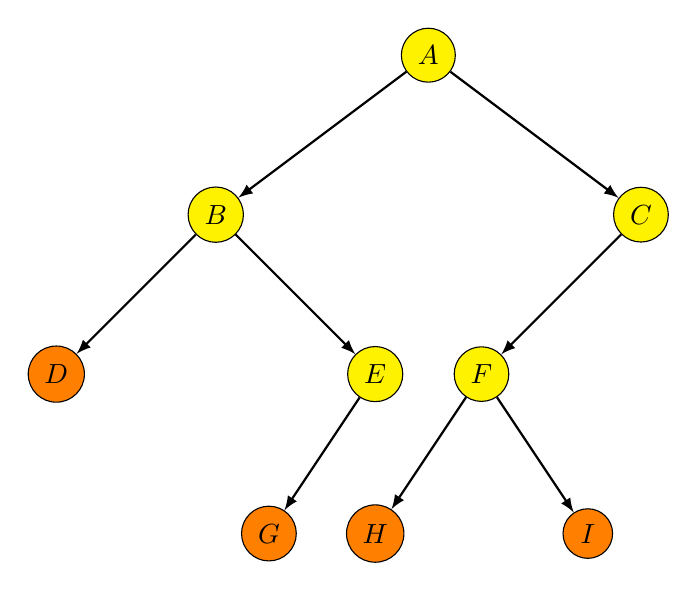
\begin{tikzpicture}[xscale=.9,yscale=.9]
% Styles (MODIFIABLES)
\tikzstyle{fleche}=[->,>=latex,thick]
\tikzstyle{nœud}=[fill=yellow,circle,draw]
\tikzstyle{feuille}=[fill=orange,circle,draw]
% Dimensions (MODIFIABLES)
\def\DistanceInterNiveaux{3}
\def\DistanceInterFeuilles{2}
% Dimensions calculées (NON MODIFIABLES)
\def\NiveauA{(-0)*\DistanceInterNiveaux}
\def\NiveauB{(-.75)*\DistanceInterNiveaux}
\def\NiveauC{(-1.5)*\DistanceInterNiveaux}
\def\NiveauD{(-2.25)*\DistanceInterNiveaux}
\def\InterFeuilles{(.75)*\DistanceInterFeuilles}
% nœuds (MODIFIABLES : Styles et Coefficients d'InterFeuilles)
\node[nœud] (R) at ({(2)*\InterFeuilles},{\NiveauA}) {$A$};
\node[nœud] (Ra) at ({(0)*\InterFeuilles},{\NiveauB}) {$B$};
\node[feuille] (Raa) at ({(-1.5)*\InterFeuilles},{\NiveauC}) {$D$};
\node[nœud] (Rab) at ({(1.5)*\InterFeuilles},{\NiveauC}) {$E$};
\node[feuille] (Raba) at ({(0.5)*\InterFeuilles},{\NiveauD}) {$G$};
\node[nœud] (Rb) at ({(4)*\InterFeuilles},{\NiveauB}) {$C$};
\node[nœud] (Rba) at ({(2.5)*\InterFeuilles},{\NiveauC}) {$F$};
\node[feuille] (Rbaa) at ({(1.5)*\InterFeuilles},{\NiveauD}) {$H$};
\node[feuille] (Rbab) at ({(3.5)*\InterFeuilles},{\NiveauD}) {$I$};
% Arcs (MODIFIABLES : Styles)
\draw[fleche] (R)--(Ra);
\draw[fleche] (Ra)--(Raa);
\draw[fleche] (Ra)--(Rab);
\draw[fleche] (Rab)--(Raba);
\draw[fleche] (R)--(Rb);
\draw[fleche] (Rb)--(Rba);
\draw[fleche] (Rba)--(Rbaa);
\draw[fleche] (Rba)--(Rbab);
\end{tikzpicture}
\end{center}
%:-+-+-+-+- Fin
\begin{multicols}{3}
Le sous-arbre gauche du nœud \code{A} est : \medskip\\

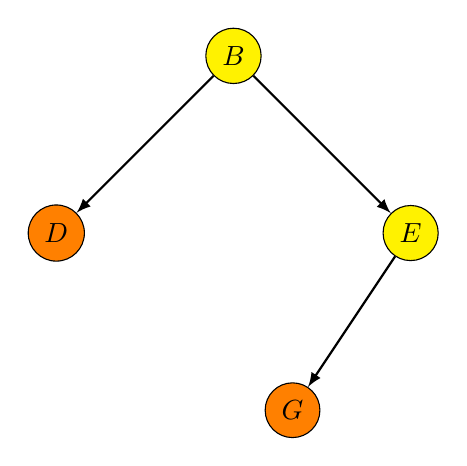
\begin{tikzpicture}[xscale=1,yscale=1]
% Styles (MODIFIABLES)
\tikzstyle{fleche}=[->,>=latex,thick]
\tikzstyle{nœud}=[fill=yellow,circle,draw]
\tikzstyle{feuille}=[fill=orange,circle,draw]
% Dimensions (MODIFIABLES)
\def\DistanceInterNiveaux{3}
\def\DistanceInterFeuilles{2}
% Dimensions calculées (NON MODIFIABLES)
\def\NiveauA{(-0)*\DistanceInterNiveaux}
\def\NiveauB{(-.75)*\DistanceInterNiveaux}
\def\NiveauC{(-1.5)*\DistanceInterNiveaux}
\def\NiveauD{(-2.25)*\DistanceInterNiveaux}
\def\InterFeuilles{(.75)*\DistanceInterFeuilles}
% nœuds (MODIFIABLES : Styles et Coefficients d'InterFeuilles)
\node[nœud] (Ra) at ({(0)*\InterFeuilles},{\NiveauB}) {$B$};
\node[feuille] (Raa) at ({(-1.5)*\InterFeuilles},{\NiveauC}) {$D$};
\node[nœud] (Rab) at ({(1.5)*\InterFeuilles},{\NiveauC}) {$E$};
\node[feuille] (Raba) at ({(0.5)*\InterFeuilles},{\NiveauD}) {$G$};
% Arcs (MODIFIABLES : Styles)
\draw[fleche] (Ra)--(Raa);
\draw[fleche] (Ra)--(Rab);
\draw[fleche] (Rab)--(Raba);
\end{tikzpicture}

Le sous-arbre droit du nœud \code{A} est : \medskip\\

% Racine en Haut, développement vers le bas
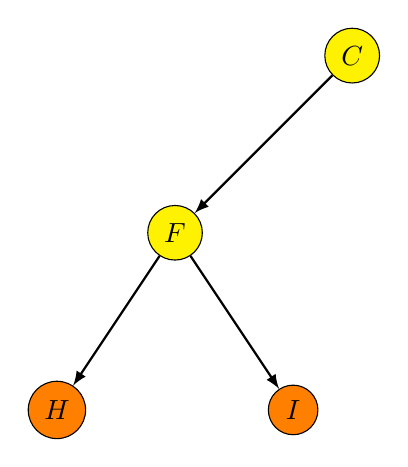
\begin{tikzpicture}[xscale=1,yscale=1]
% Styles (MODIFIABLES)
\tikzstyle{fleche}=[->,>=latex,thick]
\tikzstyle{nœud}=[fill=yellow,circle,draw]
\tikzstyle{feuille}=[fill=orange,circle,draw]
% Dimensions (MODIFIABLES)
\def\DistanceInterNiveaux{3}
\def\DistanceInterFeuilles{2}
% Dimensions calculées (NON MODIFIABLES)
\def\NiveauA{(-0)*\DistanceInterNiveaux}
\def\NiveauB{(-.75)*\DistanceInterNiveaux}
\def\NiveauC{(-1.5)*\DistanceInterNiveaux}
\def\NiveauD{(-2.25)*\DistanceInterNiveaux}
\def\InterFeuilles{(.75)*\DistanceInterFeuilles}
% nœuds (MODIFIABLES : Styles et Coefficients d'InterFeuilles)
\node[nœud] (Rb) at ({(4)*\InterFeuilles},{\NiveauB}) {$C$};
\node[nœud] (Rba) at ({(2.5)*\InterFeuilles},{\NiveauC}) {$F$};
\node[feuille] (Rbaa) at ({(1.5)*\InterFeuilles},{\NiveauD}) {$H$};
\node[feuille] (Rbab) at ({(3.5)*\InterFeuilles},{\NiveauD}) {$I$};
% Arcs (MODIFIABLES : Styles)
\draw[fleche] (Rb)--(Rba);
\draw[fleche] (Rba)--(Rbaa);
\draw[fleche] (Rba)--(Rbab);
\end{tikzpicture}

Le sous-arbre gauche du nœud \code{C} est :\medskip\\
 
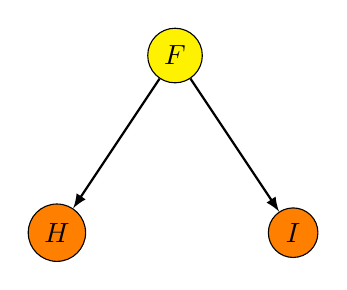
\begin{tikzpicture}[xscale=1,yscale=1]
% Styles (MODIFIABLES)
\tikzstyle{fleche}=[->,>=latex,thick]
\tikzstyle{nœud}=[fill=yellow,circle,draw]
\tikzstyle{feuille}=[fill=orange,circle,draw]
% Dimensions (MODIFIABLES)
\def\DistanceInterNiveaux{3}
\def\DistanceInterFeuilles{2}
% Dimensions calculées (NON MODIFIABLES)
\def\NiveauA{(-0)*\DistanceInterNiveaux}
\def\NiveauB{(-.75)*\DistanceInterNiveaux}
\def\NiveauC{(-1.5)*\DistanceInterNiveaux}
\def\NiveauD{(-2.25)*\DistanceInterNiveaux}
\def\InterFeuilles{(.75)*\DistanceInterFeuilles}
% nœuds (MODIFIABLES : Styles et Coefficients d'InterFeuilles)

\node[nœud] (Rba) at ({(2.5)*\InterFeuilles},{\NiveauC}) {$F$};
\node[feuille] (Rbaa) at ({(1.5)*\InterFeuilles},{\NiveauD}) {$H$};
\node[feuille] (Rbab) at ({(3.5)*\InterFeuilles},{\NiveauD}) {$I$};
% Arcs (MODIFIABLES : Styles)
\draw[fleche] (Rba)--(Rbaa);
\draw[fleche] (Rba)--(Rbab);
\end{tikzpicture}\ \\
tandis que le sous-arbre droit du nœud \code{C} est vide.
\end{multicols}\ \medskip\\
On remarque aussi que les sous-arbres gauche et droit du nœud \code{H} sont vides. Ainsi,  \code{H} est une feuille de l'arbre.

\newpage\noindent
\subsubsection*{Activité 2}
\begin{enumerate}
\item Donner les cinq structures d'arbres binaires à trois nœuds (sans étiquettes).
\item Combien existe-t-il d'arbres binaires à quatre nœuds (sans étiquettes) ?
\end{enumerate}
\vfill\noindent
\subsection*{2.2 Taille et Hauteur d'un arbre binaire}
\begin{Definition}{Taille et Hauteur d'un arbre binaire}
On appelle {\color{red} taille d'un arbre binaire} le nombre de nœuds qu'il contient.\\
On appelle {\color{red} hauteur d'un arbre binaire} le nombre maximal de nœuds rencontrés en descendant l'arbre de la racine vers une feuille.
\end{Definition}\medskip\\
Ainsi, l'arbre donné en exemple page précédente a une taille de 9 et une hauteur de 4.\\
Un arbre binaire ne contenant que sa racine est de hauteur 1.\medskip\\ 
On peut donner des inégalités simples entre la hauteur $h$ et la taille $N$ d'un arbre binaire.\\
Un arbre binaire compte au maximum :
\begin{itemize}
\item un unique nœud au niveau 1 (celui de la racine);
\item deux nœuds au niveau 2;
\item quatre nœuds au niveau 3;
\item huit nœuds au niveau 4;
\item $\ldots$
\item $2^{h-1}$ nœuds au niveau $h$, son niveau le plus haut.
\end{itemize}
Ainsi, un arbre binaire de hauteur $h$ possède au maximum $1+2+4+\cdots+2^{h-1}=2^h-1$ nœuds, c'est à dire on a $N\leq 2^h-1$.\\
Par ailleurs, si la hauteur vaut $h$, cela signifie que l'on a suivi un chemin de longueur $h$ dans l'arbre, et donc, il y au moins $h$ nœuds et donc, $h\leq N$.\\
On a donc au final : \medskip\\
\begin{Proposition}{}
Soit un arbre binaire de hauteur $h$ et la taille $N$. On a les relations 
$$h\leq N\leq 2^h-1 $$
\end{Proposition}
\subsection*{2.3 Représentation en Python}
On peut représenter un arbre binaire en Python par une structure de type chaînée, avec par exemple comme constructeur :
\begin{Python}
class nœud : 
	def __init__(self,g,v,d):
		self.gauche = g
		self.valeur = v
		self.droit = d

	def assigne_gauche(self,n):
		self.gauche = n

	def assigne_droit(self,n):
		self.droit = n
		
	def assigne_valeur(self,v):
		self.valeur = v	
\end{Python}
dans lequel :
\begin{itemize}
\item \code{v}, suivant les exemples, contient une chaîne de caractères, un type numérique, etc...
\item \code{g} et \code{d} sont des instances de la classe \code{nœud}, représentant respectivement les racines des sous-arbres gauche et droit du nœud créé, valant éventuellement \code{None} si les sous-arbres sont vides. 
\item même si on peut informatiquement affecter directement une valeur à un attribut (par exemple avec une instruction comme \code{nœudE.gauche=nœudG}), la bonne pratique en P.O.O. conseille de passer par des méthodes créées pour cela.\\
Ainsi, on fournit deux méthodes permettant de donner la racine des sous-arbres gauche et droit du nœud \code{self}. Attention, si \code{self.gauche} ou \code{self.droit} on déjà été assignés, leur contenu est écrasé et remplacé.
\end{itemize}\ \\
Par exemple, on peut créer l'arbre de racine \code{B} situé page {\bf 3} grace aux commandes : 
\begin{Python}
noeudB=noeud(None,'B',None)
noeudD=noeud(None,'D',None)
noeudE=noeud(None,'E',None)
noeudG=noeud(None,'G',None)
noeudE.assigne_gauche(noeudG)
noeudB.assigne_gauche(noeudD)
noeudB.assigne_droit(noeudE)
\end{Python}
Ici, on a d'abord créé les nœuds indépendamment puis on les a attachés; c'est une construction ''par la racine''. \\
On peut proposer une autre manière de faire dans laquelle on construit d'abord les nœuds feuilles.
\begin{Python}
noeudD=noeud(None,'D',None)
noeudG=noeud(None,'G',None)
noeudE=noeud(noeudG,'E',None)
noeudB=noeud(noeudD,'B',noeudE)
\end{Python}
Cette manière de faire est plus simple mais ne se justifie que dans une situation où il est logique de commencer à créer l'arbre par ses feuilles. 
\subsubsection*{Activité 3}
Compléter les codes Python ci-dessus pour créer des deux manières (''par la racine'' et ''par les feuilles'') l'arbre au complet. 

\newpage\noindent
\section*{\vskip -8mm 3 Algorithme sur les arbres binaires}
Les structures d'arbres se prêtent particulièrement bien à l'écriture d'algorithmes récursifs.
\subsection*{\vskip -7mm 3.1 Taille}
\begin{Python}
def taille(noeud):
	if noeud is None :
		return 0
	else :
		return 1+taille(noeud.gauche)+taille(noeud.droit)
\end{Python} 
Par exemple, quand on applique cet algorithme à l'arbre :

% Racine en Haut, développement vers le bas
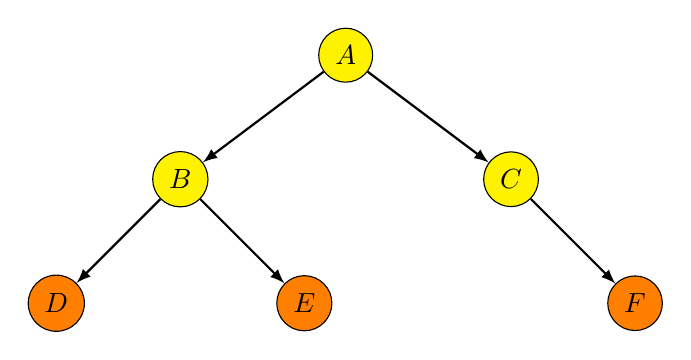
\begin{tikzpicture}[xscale=.7,yscale=.7]
% Styles (MODIFIABLES)
\tikzstyle{fleche}=[->,>=latex,thick]
\tikzstyle{nœud}=[fill=yellow,circle,draw]
\tikzstyle{feuille}=[fill=orange,circle,draw]
% Dimensions (MODIFIABLES)
\def\DistanceInterNiveaux{3}
\def\DistanceInterFeuilles{2}
% Dimensions calculées (NON MODIFIABLES)
\def\NiveauA{(-0)*\DistanceInterNiveaux}
\def\NiveauB{(-.75)*\DistanceInterNiveaux}
\def\NiveauC{(-1.5)*\DistanceInterNiveaux}
\def\NiveauD{(-2.25)*\DistanceInterNiveaux}
\def\InterFeuilles{(.75)*\DistanceInterFeuilles}
% nœuds (MODIFIABLES : Styles et Coefficients d'InterFeuilles)
\node[nœud] (R) at ({(2)*\InterFeuilles},{\NiveauA}) {$A$};
\node[nœud] (Ra) at ({(0)*\InterFeuilles},{\NiveauB}) {$B$};
\node[feuille] (Raa) at ({(-1.5)*\InterFeuilles},{\NiveauC}) {$D$};
\node[feuille] (Rab) at ({(1.5)*\InterFeuilles},{\NiveauC}) {$E$};
\node[nœud] (Rb) at ({(4)*\InterFeuilles},{\NiveauB}) {$C$};
\node[feuille] (Rba) at ({(5.5)*\InterFeuilles},{\NiveauC}) {$F$};
% Arcs (MODIFIABLES : Styles)
\draw[fleche] (R)--(Ra);
\draw[fleche] (Ra)--(Raa);
\draw[fleche] (Ra)--(Rab);
\draw[fleche] (R)--(Rb);
\draw[fleche] (Rb)--(Rba);

\end{tikzpicture}
%:-+-+-+-+- Fin
\medskip\\
Le déroulement de l'exécution de la fonction est le suivant :\\
\code{noeudA} n'est pas \code{None} et \code{noeudA.gauche=noeudB} et \code{noeudA.droit=noeudC}\\
Donc \code{taille(noeudA)} renvoie \code{1+taille(noeudB)+taille(noeudC)}
\begin{itemize}
\item \code{noeudB} n'est pas \code{None} et \code{noeudB.gauche=noeudD} et \code{noeudB.droit=noeudE}\\
Donc \code{taille(noeudB)} renvoie \code{1+taille(noeudD)+taille(noeudE)}
\begin{itemize}
\item \code{noeudD} n'est pas \code{None} et \code{noeudD.gauche=None} et \code{noeudD.droit=None}.\\
Donc \code{taille(noeudD)} renvoie \code{1+taille(None)+taille(None)=1+0+0=1}
\item \code{noeudE} n'est pas \code{None} et \code{noeudE.gauche=None} et \code{noeudE.droit=None}\\
Donc \code{taille(noeudE)} renvoie \code{1+taille(None)+taille(None)=1+0+0=1}
\end{itemize}
Donc \code{taille(noeudB)=1+1+1=3}
\item \code{noeudC} n'est pas \code{None} et \code{noeudC.gauche=None} et \code{noeudC.droit=noeudF}\\
Donc \code{taille(noeudC)} renvoie \code{1+taille(None)+taille(noeudF)=1+0+taille(noeudF)}
\begin{itemize}
\item \code{noeudF} n'est pas \code{None} et \code{noeudF.gauche=None} et \code{noeudF.droit=None}\\
Donc \code{taille(noeudF)} renvoie \code{1+taille(None)+taille(None)=1+0+0=1}
\end{itemize}
Donc \code{taille(noeudC)=1+0+1=2}
\end{itemize}
Donc, \code{taille(noeudA)=1+3+2=6}
\medskip\\
On constate qu'avec cet algorithme : 
\begin{itemize}
\item Le cas terminal est le nœud vide, pour lequel la fonction renvoie $0$.
\item Le cas particulier suivant est celui des feuilles, pour lequel la fonction renvoie $1+0+0=1$.
\item La fonction, appliquée à un nœud \code{n} renvoie 1 + nombre de nœuds présents sur l'arbre gauche de \code{n} + nombre de nœuds présents sur l'arbre droit de \code{n}.
\end{itemize}
{\bf Remarque : }On constate donc bien le bon fonctionnement de l'algorithme, que l'on peut visualiser de manière plus simple en commençant par assigner le nombre \code{1} à chaque feuille, puis, en remontant, en assignant à chaque nœud le nombre \code{1}+la somme des valeurs de ses nœuds enfants.
%\newpage\noindent
\subsection*{3.2 Hauteur}
\begin{Python}
def hauteur(noeud):
	if noeud is None :
		return 0
	else :
		return 1+max(hauteur(noeud.gauche),hauteur(noeud.droit))
\end{Python} 
On constate qu'avec cet algorithme : 
\begin{itemize}
\item Le cas terminal est le nœud vide, pour lequel la fonction renvoie $0$.
\item Le cas particulier suivant est celui des feuilles, pour lequel la fonction renvoie $1+\max(0,0)=1$.
\end{itemize}
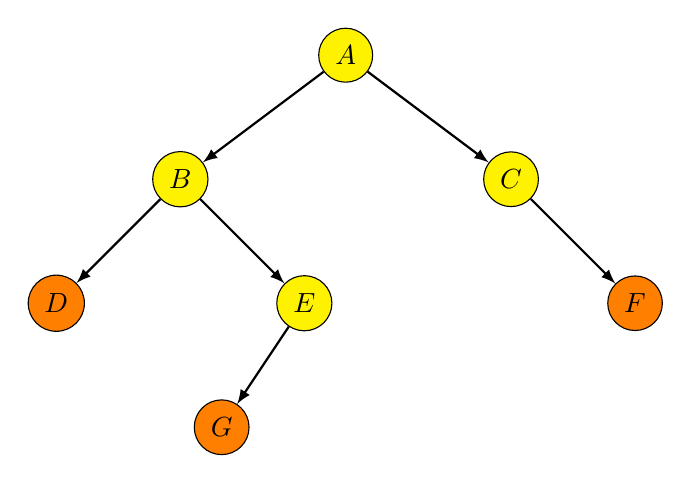
\begin{tikzpicture}[xscale=.7,yscale=.7]
% Styles (MODIFIABLES)
\tikzstyle{fleche}=[->,>=latex,thick]
\tikzstyle{nœud}=[fill=yellow,circle,draw]
\tikzstyle{feuille}=[fill=orange,circle,draw]
% Dimensions (MODIFIABLES)
\def\DistanceInterNiveaux{3}
\def\DistanceInterFeuilles{2}
% Dimensions calculées (NON MODIFIABLES)
\def\NiveauA{(-0)*\DistanceInterNiveaux}
\def\NiveauB{(-.75)*\DistanceInterNiveaux}
\def\NiveauC{(-1.5)*\DistanceInterNiveaux}
\def\NiveauD{(-2.25)*\DistanceInterNiveaux}
\def\InterFeuilles{(.75)*\DistanceInterFeuilles}
% nœuds (MODIFIABLES : Styles et Coefficients d'InterFeuilles)
\node[nœud] (R) at ({(2)*\InterFeuilles},{\NiveauA}) {$A$};
\node[nœud] (Ra) at ({(0)*\InterFeuilles},{\NiveauB}) {$B$};
\node[feuille] (Raa) at ({(-1.5)*\InterFeuilles},{\NiveauC}) {$D$};
\node[nœud] (Rab) at ({(1.5)*\InterFeuilles},{\NiveauC}) {$E$};
\node[feuille] (Raba) at ({(0.5)*\InterFeuilles},{\NiveauD}) {$G$};
\node[nœud] (Rb) at ({(4)*\InterFeuilles},{\NiveauB}) {$C$};
\node[feuille] (Rba) at ({(5.5)*\InterFeuilles},{\NiveauC}) {$F$};
% Arcs (MODIFIABLES : Styles)
\draw[fleche] (R)--(Ra);
\draw[fleche] (Ra)--(Raa);
\draw[fleche] (Ra)--(Rab);
\draw[fleche] (Rab)--(Raba);
\draw[fleche] (R)--(Rb);
\draw[fleche] (Rb)--(Rba);
\end{tikzpicture}
\medskip\\
Si on applique la fonction \code{hauteur} à l'arbre ci-dessus, on obtient : \medskip\\
\code{hauteur(noeudA)=1+max(hauteur(noeudB),hauteur(noeudC))}
\begin{itemize}
\item \code{hauteur(noeudB)=1+max(hauteur(noeudD),hauteur(noeudE))}
         \begin{itemize}
          \item \code{hauteur(noeudD)=1+max(hauteur(None),hauteur(None))=1+0=1}
          \item\code{hauteur(noeudE)=1+max(hauteur(noeudG),hauteur(None))=1+hauteur(noeudG)}
                   \begin{itemize}
                    \item \code{hauteur(noeudG)=1+max(hauteur(None),hauteur(None))=1+0=1}
                    \end{itemize}
                    Donc \code{hauteur(noeudE)=1+1=2}
          \end{itemize}
          Donc \code{hauteur(noeudB)=1+max(1,2)=1+2=3}
\item \code{hauteur(noeudC)=1+max(hauteur(None),hauteur(noeudF))=1+hauteur(noeudF)}
         \begin{itemize}
          \item \code{hauteur(noeudF)=1+max(hauteur(None),hauteur(None))=1+0=1}
          \end{itemize}
          Donc \code{hauteur(noeudC)=1+1=2}
\end{itemize}
Donc \code{hauteur(noeudA)=1+max(3,2)=1+3=4}\medskip\\
{\bf Remarque : }Là encore, on peut visualiser le fonctionnement de cet algorithme de manière plus simple en commençant par assigner le nombre \code{1} à chaque feuille, puis, en remontant, en assignant à chaque nœud le nombre \code{1}+le max des valeurs de ses nœuds enfants.

\newpage
\subsubsection*{Activité 4}
En utilisant les deux remarques ci-dessus, visualisez le fonctionnement des algorithmes de calcul de taille et de hauteur appliqués à l'arbre binaire suivant  :\medskip\\
% Racine en Haut, développement vers le bas
\begin{center}
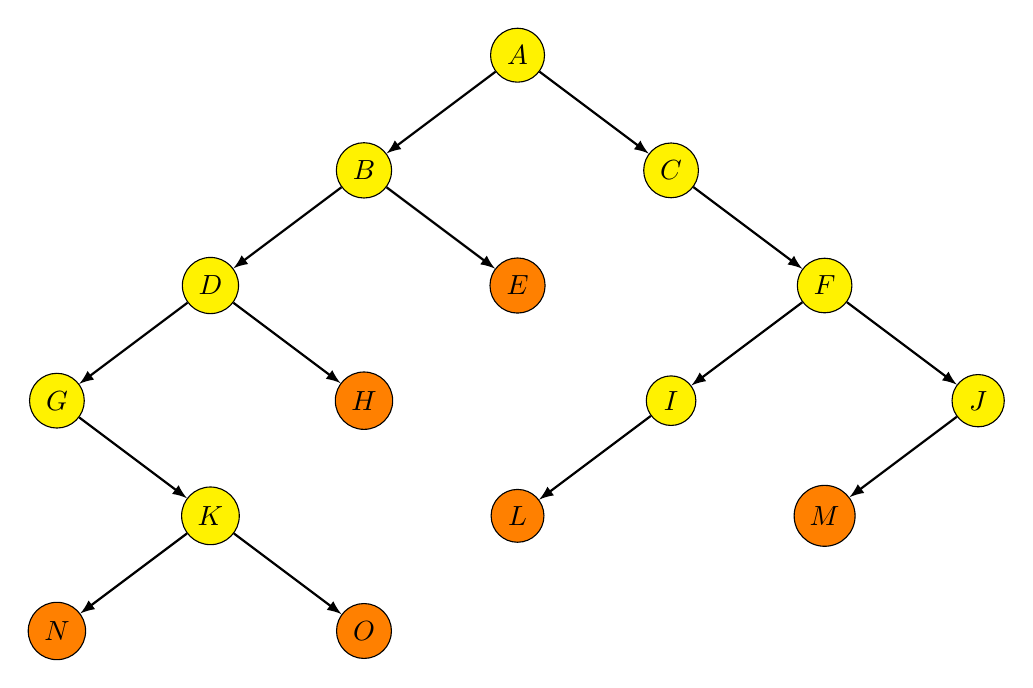
\begin{tikzpicture}[xscale=.65,yscale=.65]
% Styles (MODIFIABLES)
\tikzstyle{fleche}=[->,>=latex,thick]
\tikzstyle{nœud}=[fill=yellow,circle,draw]
\tikzstyle{feuille}=[fill=orange,circle,draw]
% Dimensions (MODIFIABLES)
\def\DistanceInterNiveaux{3}
\def\DistanceInterFeuilles{2}
% Dimensions calculées (NON MODIFIABLES)
\def\NiveauA{(-0)*\DistanceInterNiveaux}
\def\NiveauB{(-.75)*\DistanceInterNiveaux}
\def\NiveauC{(-1.5)*\DistanceInterNiveaux}
\def\NiveauD{(-2.25)*\DistanceInterNiveaux}
\def\NiveauE{(-3)*\DistanceInterNiveaux}
\def\NiveauF{(-3.75)*\DistanceInterNiveaux}
\def\InterFeuilles{(.75)*\DistanceInterFeuilles}
% nœuds (MODIFIABLES : Styles et Coefficients d'InterFeuilles)
\node[nœud] (R) at ({(0)*\InterFeuilles},{\NiveauA}) {$A$};
\node[nœud] (Ra) at ({(-2)*\InterFeuilles},{\NiveauB}) {$B$};
\node[nœud] (Rb) at ({(2)*\InterFeuilles},{\NiveauB}) {$C$};
\node[nœud] (Raa) at ({(-4)*\InterFeuilles},{\NiveauC}) {$D$};
\node[feuille] (Rab) at ({(0)*\InterFeuilles},{\NiveauC}) {$E$};
\node[nœud] (Rbb) at ({(4)*\InterFeuilles},{\NiveauC}) {$F$};
\node[nœud] (Raaa) at ({(-6)*\InterFeuilles},{\NiveauD}) {$G$};
\node[feuille] (Raab) at ({(-2)*\InterFeuilles},{\NiveauD}) {$H$};
\node[nœud] (Rbba) at ({(2)*\InterFeuilles},{\NiveauD}) {$I$};
\node[nœud] (Rbbb) at ({(6)*\InterFeuilles},{\NiveauD}) {$J$};
\node[nœud] (Raaab) at ({(-4)*\InterFeuilles},{\NiveauE}) {$K$};
\node[feuille] (Rbbaa) at ({(0)*\InterFeuilles},{\NiveauE}) {$L$};
\node[feuille] (Rbbba) at ({(4)*\InterFeuilles},{\NiveauE}) {$M$};
\node[feuille] (Raaaba) at ({(-6)*\InterFeuilles},{\NiveauF}) {$N$};
\node[feuille] (Raaabb) at ({(-2)*\InterFeuilles},{\NiveauF}) {$O$};
% Arcs (MODIFIABLES : Styles)
\draw[fleche] (R)--(Ra);
\draw[fleche] (R)--(Rb);
\draw[fleche] (Ra)--(Raa);
\draw[fleche] (Ra)--(Rab);
\draw[fleche] (Rb)--(Rbb);
\draw[fleche] (Raa)--(Raaa);
\draw[fleche] (Raa)--(Raab);
\draw[fleche] (Rbb)--(Rbba);
\draw[fleche] (Rbb)--(Rbbb);
\draw[fleche] (Raaa)--(Raaab);
\draw[fleche] (Rbba)--(Rbbaa);
\draw[fleche] (Rbbb)--(Rbbba);
\draw[fleche] (Raaab)--(Raaaba);
\draw[fleche] (Raaab)--(Raaabb);

\end{tikzpicture}
\end{center}
%:-+-+-+-+- Fin

\newpage\noindent
\subsection*{3.3 Parcours d'arbres en profondeur}
\subsubsection*{3.3.1 Définitions}
\begin{Definition}{Parcours d'arbres en profondeur}
Un parcours d'arbre est un processus qui part d'un nœud et visite les nœuds de l'arbre une unique fois.\\
%TODO : définition d'un parcours en profondeur d'un graphe.
On distingue :   
\begin{enumerate}
\item le parcours infixe : c'est un parcours dans lequel pour chaque nœud \code{n} de l'arbre et de manière récursive, on liste :
\begin{itemize}
\item tous les nœuds de l'arbre gauche de \code{n}
\item le nœud \code{n}
\item tous les nœuds de l'arbre droit de \code{n}
\end{itemize}
\item le parcours préfixe : c'est un parcours dans lequel pour chaque nœud \code{n} de l'arbre et de manière récursive, on liste :
\begin{itemize}
\item le nœud \code{n}
\item tous les nœuds de l'arbre gauche de \code{n}
\item tous les nœuds de l'arbre droit de \code{n}
\end{itemize}
\item le parcours suffixe : c'est un parcours dans lequel pour chaque nœud \code{n} de l'arbre et de manière récursive, on liste :
\begin{itemize}
\item tous les nœuds de l'arbre gauche de \code{n}
\item tous les nœuds de l'arbre droit de \code{n}
\item le nœud \code{n}
\end{itemize}
\end{enumerate}
\end{Definition} \medskip\\
Pour une première illustration, 
\begin{multicols}{2}
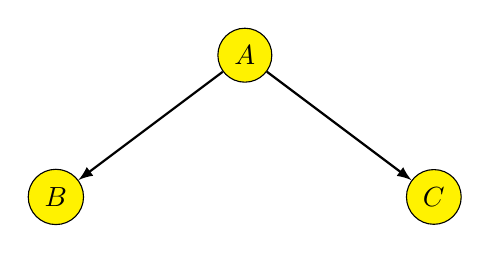
\begin{tikzpicture}[xscale=.8,yscale=.8]
% Styles (MODIFIABLES)
\tikzstyle{fleche}=[->,>=latex,thick]
\tikzstyle{nœud}=[fill=yellow,circle,draw]
\tikzstyle{feuille}=[fill=orange,circle,draw]
% Dimensions (MODIFIABLES)
\def\DistanceInterNiveaux{3}
\def\DistanceInterFeuilles{2}
% Dimensions calculées (NON MODIFIABLES)
\def\NiveauA{(-0)*\DistanceInterNiveaux}
\def\NiveauB{(-.75)*\DistanceInterNiveaux}
\def\NiveauC{(-1.5)*\DistanceInterNiveaux}
\def\NiveauD{(-2.25)*\DistanceInterNiveaux}
\def\InterFeuilles{(.75)*\DistanceInterFeuilles}
% nœuds (MODIFIABLES : Styles et Coefficients d'InterFeuilles)
\node[nœud] (R) at ({(2)*\InterFeuilles},{\NiveauA}) {$A$};
\node[nœud] (Ra) at ({(0)*\InterFeuilles},{\NiveauB}) {$B$};
\node[nœud] (Rb) at ({(4)*\InterFeuilles},{\NiveauB}) {$C$};
% Arcs (MODIFIABLES : Styles)
\draw[fleche] (R)--(Ra);
\draw[fleche] (R)--(Rb);
\end{tikzpicture}

Le parcours infixe donne \code{B-A-C}\\
Le parcours préfixe donne \code{A-B-C}\\
Le parcours suffixe donne \code{B-C-A}
\end{multicols}

On va maintenant étudier ces trois types de parcours sur l'exemple suivant : 
\begin{center}
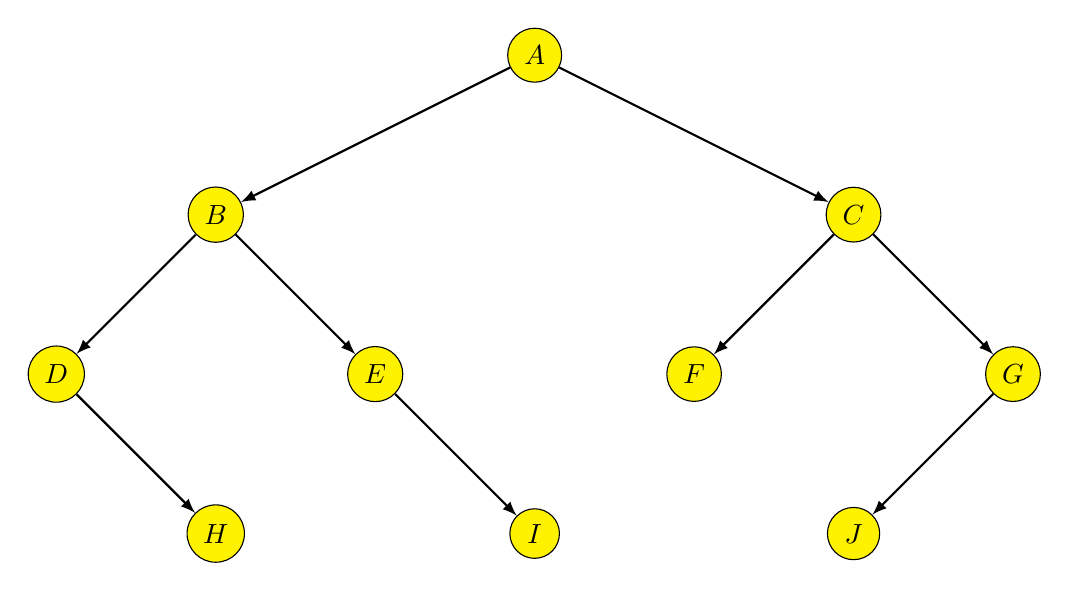
\begin{tikzpicture}[xscale=.9,yscale=.9]
% Styles (MODIFIABLES)
\tikzstyle{fleche}=[->,>=latex,thick]
\tikzstyle{nœud}=[fill=yellow,circle,draw]
\tikzstyle{feuille}=[fill=orange,circle,draw]
% Dimensions (MODIFIABLES)
\def\DistanceInterNiveaux{3}
\def\DistanceInterFeuilles{2}
% Dimensions calculées (NON MODIFIABLES)
\def\NiveauA{(-0)*\DistanceInterNiveaux}
\def\NiveauB{(-.75)*\DistanceInterNiveaux}
\def\NiveauC{(-1.5)*\DistanceInterNiveaux}
\def\NiveauD{(-2.25)*\DistanceInterNiveaux}
\def\InterFeuilles{(.75)*\DistanceInterFeuilles}
% nœuds (MODIFIABLES : Styles et Coefficients d'InterFeuilles)
\node[nœud] (R) at ({(3)*\InterFeuilles},{\NiveauA}) {$A$};
\node[nœud] (Ra) at ({(0)*\InterFeuilles},{\NiveauB}) {$B$};
\node[nœud] (Rb) at ({(6)*\InterFeuilles},{\NiveauB}) {$C$};
\node[nœud] (Raa) at ({(-1.5)*\InterFeuilles},{\NiveauC}) {$D$};
\node[nœud] (Rab) at ({(1.5)*\InterFeuilles},{\NiveauC}) {$E$};
\node[nœud] (Rba) at ({(4.5)*\InterFeuilles},{\NiveauC}) {$F$};
\node[nœud] (Rbb) at ({(7.5)*\InterFeuilles},{\NiveauC}) {$G$};
\node[nœud] (Raaa) at ({(0)*\InterFeuilles},{\NiveauD}) {$H$};
\node[nœud] (Rabb) at ({(3)*\InterFeuilles},{\NiveauD}) {$I$};
\node[nœud] (Rbbb) at ({(6)*\InterFeuilles},{\NiveauD}) {$J$};
% Arcs (MODIFIABLES : Styles)
\draw[fleche] (R)--(Ra);
\draw[fleche] (R)--(Rb);
\draw[fleche] (Ra)--(Raa);
\draw[fleche] (Ra)--(Rab);
\draw[fleche] (Rb)--(Rba);
\draw[fleche] (Rb)--(Rbb);
\draw[fleche] (Raa)--(Raaa);
\draw[fleche] (Rab)--(Rabb);
\draw[fleche] (Rbb)--(Rbbb);
\end{tikzpicture}
\end{center}
Dans la suite, pour faciliter l'écriture, on nomme \code{A} le nœud de valeur \code{'A'}.
\subsubsection*{3.3.2 Parcours infixe}
Dans ce parcours, un nœud est visité après que tous les nœuds de son arbre gauche aient été visités et avant que n'importe quel nœud de son arbre droit n'ait été visité.  
\begin{Python}
def parcours_infixe(noeud):
	'''argument  : un nœud possédant une valeur de type str 
	résultat : un type str '''  
	if noeud is None :
		return ''
	else :
		return parcours_infixe(noeud.gauche)+' '+noeud.valeur+' '+parcours_infixe(noeud.droit)
\end{Python} 
(Dans la suite, on note \code{p\_i} pour la fonction \code{parcours\_infixe} .)\\
Le parcours infixe à partir de \code{A} donne le résultat :\\
\centerline{\code{'D H B E I A F C J G'}} \\
En effet, le premier appel récursif renvoie :\\
\centerline{\code{p\_i(B)+' '+'A'+' '+p\_i(C)}}\\
Donc, dans le résultat final, tous les nœuds de l'arbre gauche de \code{A} (c'est à dire \code{B}, \code{D}, \code{E}, \code{H}, \code{I}) seront à gauche de \code{A} et que tous les nœuds de l'arbre droit de \code{A} (c'est à dire \code{C}, \code{F}, \code{G}, \code{J}) seront à droite de \code{A}.\\
Comment classer \code{B}, \code{D}, \code{E}, \code{H}, \code{I} entre eux ? \\
Le deuxième appel récursif renvoie :\\
\centerline{\code{p\_i(D)+' '+'B'+' '+p\_i(E)}}\\
Donc, dans le résultat final, les nœuds de l'arbre gauche de \code{B} (c'est à dire \code{D} et \code{H}) seront à gauche de \code{B} et les nœuds de l'arbre droit de \code{B} (c'est à dire \code{E}, \code{I}) seront à droite de \code{B}.\\
Pour la suite, \code{D.gauche} est vide et \code{D.droit} est la feuille \code{H}, donc l'appel \code{p\_i(D)} renvoie \code{'D H'}, etc.\\
On remarque de même que \code{G.gauche} est la feuille \code{J} et \code{G.droit} est vide, donc l'appel \code{p\_i(G)} renvoie \code{'J G'}.
%
%%
%
\subsubsection*{3.3.3 Parcours préfixe}
Dans ce parcours, un nœud est visité avant que n'importe lequel de ses enfants n'ait été visité.  
\begin{Python}
def parcours_prefixe(noeud):
	'''argument  : un noeud possédant une valeur de type str 
	résultat : un type str '''  
	if noeud is None :
		return ''
	else :
		return noeud.valeur+' '+parcours_prefixe(noeud.gauche)+' '+parcours_prefixe(noeud.droit)
\end{Python} 
(Dans la suite, on note \code{p\_p} pour la fonction \code{parcours\_prefixe} .)\\
Le parcours préfixe à partir de \code{A} donne le résultat :\\
\centerline{\code{'A B D H E I C F G J'}} \\
En effet, le premier appel récursif renvoie :\\
\centerline{\code{'A'+' '+p\_p(B)+' '+p\_p(C)}}\\
Donc, dans le résultat final, \code{A} sera en premier, suivi de tous les nœuds de l'arbre gauche de \code{A} (c'est à dire \code{B}, \code{D}, \code{E}, \code{H}, \code{I}) eux mêmes suivis de tous les nœuds de l'arbre droit de \code{A} (c'est à dire \code{C}, \code{F}, \code{G}, \code{J}).\\
Comment classer \code{B}, \code{D}, \code{E}, \code{H}, \code{I} entre eux ? \\
Le deuxième appel récursif renvoie :\\
\centerline{\code{'B'+' '+p\_p(D)+' '+p\_p(E)}}\\
Donc, dans le résultat final, \code{B} sera suivi par les nœuds de l'arbre gauche de \code{B} (c'est à dire \code{D} et \code{H}) eux mêmes suivis de tous les nœuds de l'arbre droit de \code{B} (c'est à dire \code{E}, \code{I}) .\\
Pour la suite, \code{D.gauche} est vide et \code{D.droit} est la feuille \code{H}, donc l'appel \code{p\_p(D)} renvoie \code{'D H'}, etc..\\
On remarque de même que \code{G.gauche} est la feuille \code{J} et \code{G.droit} est vide, donc l'appel \code{p\_p(G)} renvoie \code{'G J'}.

\subsubsection*{3.3.4 Parcours suffixe}
Dans ce parcours, un nœud est visité après que tous ses enfants aient été visités.  

\begin{Python}
def parcours_suffixe(noeud):
	'''argument  : un nœud possédant une valeur de type str
	résultat : un type str '''  
	if noeud is None :
		return ''
	else :
		return parcours_suffixe(noeud.gauche)+' '+parcours_suffixe(noeud.droit)+' '+noeud.valeur
\end{Python} 
(Dans la suite, on note \code{p\_s} pour la fonction \code{parcours\_suffixe} .)\\
Le parcours suffixe à partir de \code{A} donne le résultat :\\
\centerline{\code{'H D I E B F J G C A'}} \\
En effet, le premier appel récursif renvoie :\\
\centerline{\code{p\_s(B)+' '+p\_s(C)+' '+'A'}}\\
Donc, dans le résultat final, on aura d'abord tous les nœuds de l'arbre gauche de \code{A} (c'est à dire \code{B}, \code{D}, \code{E}, \code{H}, \code{I}) suivis de tous les nœuds de l'arbre droit de \code{A} (c'est à dire \code{C}, \code{F}, \code{G}, \code{J}) et enfin, on aura \code{A}.\\
Comment classer \code{B}, \code{D}, \code{E}, \code{H}, \code{I} entre eux ? \\
Le deuxième appel récursif renvoie :\\
\centerline{\code{p\_s(D)+' '+p\_s(E)+' '+'B'}}\\
Donc, dans le résultat final, les nœuds de l'arbre gauche de \code{B} (c'est à dire \code{D} et \code{H}) seront suivis des nœuds de l'arbre droit de \code{B} (c'est à dire \code{E}, \code{I}) qui seront suivis de \code{B}.\\
Pour la suite, \code{D.gauche} est vide et \code{D.droit} est la feuille \code{H}, donc l'appel \code{p\_s(D)} renvoie \code{'D H'}, etc.\\
On remarque de même que \code{G.gauche} est la feuille \code{J} et \code{G.droit} est vide, donc l'appel \code{p\_s(G)} renvoie \code{'J G'}.
\subsubsection*{Activité 5}
Donner les parcours infixes, suffixes et préfixes des arbres suivants : 
\begin{enumerate}
\item Arbre 2 \medskip\\
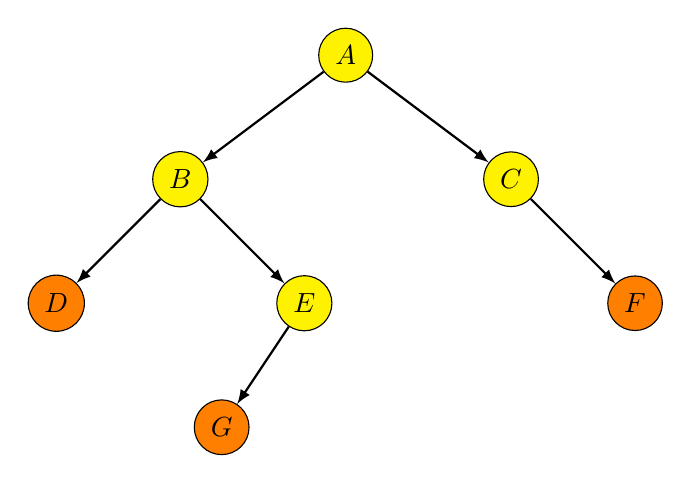
\begin{tikzpicture}[xscale=.7,yscale=.7]
% Styles (MODIFIABLES)
\tikzstyle{fleche}=[->,>=latex,thick]
\tikzstyle{nœud}=[fill=yellow,circle,draw]
\tikzstyle{feuille}=[fill=orange,circle,draw]
% Dimensions (MODIFIABLES)
\def\DistanceInterNiveaux{3}
\def\DistanceInterFeuilles{2}
% Dimensions calculées (NON MODIFIABLES)
\def\NiveauA{(-0)*\DistanceInterNiveaux}
\def\NiveauB{(-.75)*\DistanceInterNiveaux}
\def\NiveauC{(-1.5)*\DistanceInterNiveaux}
\def\NiveauD{(-2.25)*\DistanceInterNiveaux}
\def\InterFeuilles{(.75)*\DistanceInterFeuilles}
% nœuds (MODIFIABLES : Styles et Coefficients d'InterFeuilles)
\node[nœud] (R) at ({(2)*\InterFeuilles},{\NiveauA}) {$A$};
\node[nœud] (Ra) at ({(0)*\InterFeuilles},{\NiveauB}) {$B$};
\node[feuille] (Raa) at ({(-1.5)*\InterFeuilles},{\NiveauC}) {$D$};
\node[nœud] (Rab) at ({(1.5)*\InterFeuilles},{\NiveauC}) {$E$};
\node[feuille] (Raba) at ({(0.5)*\InterFeuilles},{\NiveauD}) {$G$};
\node[nœud] (Rb) at ({(4)*\InterFeuilles},{\NiveauB}) {$C$};
\node[feuille] (Rba) at ({(5.5)*\InterFeuilles},{\NiveauC}) {$F$};
% Arcs (MODIFIABLES : Styles)
\draw[fleche] (R)--(Ra);
\draw[fleche] (Ra)--(Raa);
\draw[fleche] (Ra)--(Rab);
\draw[fleche] (Rab)--(Raba);
\draw[fleche] (R)--(Rb);
\draw[fleche] (Rb)--(Rba);
\end{tikzpicture}
\newpage\noindent
\item Arbre 1 \medskip\\
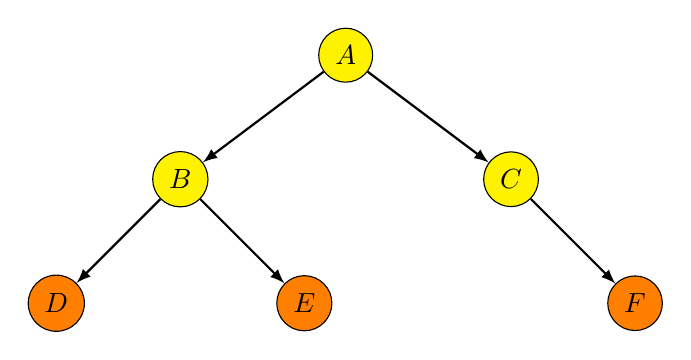
\begin{tikzpicture}[xscale=.7,yscale=.7]
% Styles (MODIFIABLES)
\tikzstyle{fleche}=[->,>=latex,thick]
\tikzstyle{nœud}=[fill=yellow,circle,draw]
\tikzstyle{feuille}=[fill=orange,circle,draw]
% Dimensions (MODIFIABLES)
\def\DistanceInterNiveaux{3}
\def\DistanceInterFeuilles{2}
% Dimensions calculées (NON MODIFIABLES)
\def\NiveauA{(-0)*\DistanceInterNiveaux}
\def\NiveauB{(-.75)*\DistanceInterNiveaux}
\def\NiveauC{(-1.5)*\DistanceInterNiveaux}
\def\NiveauD{(-2.25)*\DistanceInterNiveaux}
\def\InterFeuilles{(.75)*\DistanceInterFeuilles}
% nœuds (MODIFIABLES : Styles et Coefficients d'InterFeuilles)
\node[nœud] (R) at ({(2)*\InterFeuilles},{\NiveauA}) {$A$};
\node[nœud] (Ra) at ({(0)*\InterFeuilles},{\NiveauB}) {$B$};
\node[feuille] (Raa) at ({(-1.5)*\InterFeuilles},{\NiveauC}) {$D$};
\node[feuille] (Rab) at ({(1.5)*\InterFeuilles},{\NiveauC}) {$E$};
\node[nœud] (Rb) at ({(4)*\InterFeuilles},{\NiveauB}) {$C$};
\node[feuille] (Rba) at ({(5.5)*\InterFeuilles},{\NiveauC}) {$F$};
% Arcs (MODIFIABLES : Styles)
\draw[fleche] (R)--(Ra);
\draw[fleche] (Ra)--(Raa);
\draw[fleche] (Ra)--(Rab);
\draw[fleche] (R)--(Rb);
\draw[fleche] (Rb)--(Rba);

\end{tikzpicture}
\ \\ \\ \\ \\ \\ \\\\ \\
\item Arbre 3 \medskip\\
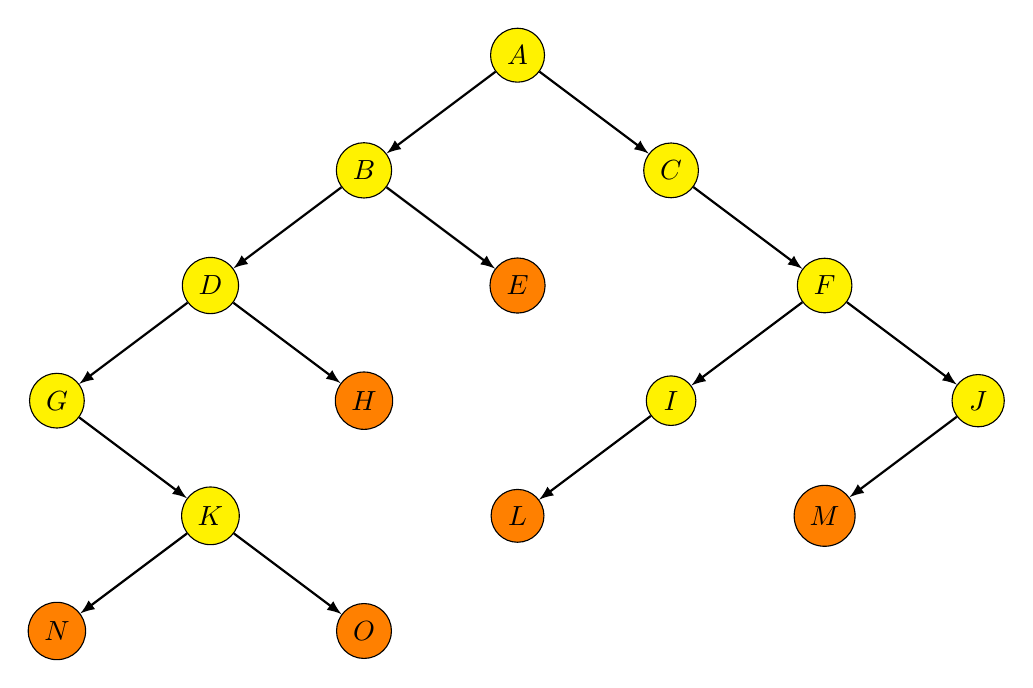
\begin{tikzpicture}[xscale=.65,yscale=.65]
% Styles (MODIFIABLES)
\tikzstyle{fleche}=[->,>=latex,thick]
\tikzstyle{nœud}=[fill=yellow,circle,draw]
\tikzstyle{feuille}=[fill=orange,circle,draw]
% Dimensions (MODIFIABLES)
\def\DistanceInterNiveaux{3}
\def\DistanceInterFeuilles{2}
% Dimensions calculées (NON MODIFIABLES)
\def\NiveauA{(-0)*\DistanceInterNiveaux}
\def\NiveauB{(-.75)*\DistanceInterNiveaux}
\def\NiveauC{(-1.5)*\DistanceInterNiveaux}
\def\NiveauD{(-2.25)*\DistanceInterNiveaux}
\def\NiveauE{(-3)*\DistanceInterNiveaux}
\def\NiveauF{(-3.75)*\DistanceInterNiveaux}
\def\InterFeuilles{(.75)*\DistanceInterFeuilles}
% nœuds (MODIFIABLES : Styles et Coefficients d'InterFeuilles)
\node[nœud] (R) at ({(0)*\InterFeuilles},{\NiveauA}) {$A$};
\node[nœud] (Ra) at ({(-2)*\InterFeuilles},{\NiveauB}) {$B$};
\node[nœud] (Rb) at ({(2)*\InterFeuilles},{\NiveauB}) {$C$};
\node[nœud] (Raa) at ({(-4)*\InterFeuilles},{\NiveauC}) {$D$};
\node[feuille] (Rab) at ({(0)*\InterFeuilles},{\NiveauC}) {$E$};
\node[nœud] (Rbb) at ({(4)*\InterFeuilles},{\NiveauC}) {$F$};
\node[nœud] (Raaa) at ({(-6)*\InterFeuilles},{\NiveauD}) {$G$};
\node[feuille] (Raab) at ({(-2)*\InterFeuilles},{\NiveauD}) {$H$};
\node[nœud] (Rbba) at ({(2)*\InterFeuilles},{\NiveauD}) {$I$};
\node[nœud] (Rbbb) at ({(6)*\InterFeuilles},{\NiveauD}) {$J$};
\node[nœud] (Raaab) at ({(-4)*\InterFeuilles},{\NiveauE}) {$K$};
\node[feuille] (Rbbaa) at ({(0)*\InterFeuilles},{\NiveauE}) {$L$};
\node[feuille] (Rbbba) at ({(4)*\InterFeuilles},{\NiveauE}) {$M$};
\node[feuille] (Raaaba) at ({(-6)*\InterFeuilles},{\NiveauF}) {$N$};
\node[feuille] (Raaabb) at ({(-2)*\InterFeuilles},{\NiveauF}) {$O$};
% Arcs (MODIFIABLES : Styles)
\draw[fleche] (R)--(Ra);
\draw[fleche] (R)--(Rb);
\draw[fleche] (Ra)--(Raa);
\draw[fleche] (Ra)--(Rab);
\draw[fleche] (Rb)--(Rbb);
\draw[fleche] (Raa)--(Raaa);
\draw[fleche] (Raa)--(Raab);
\draw[fleche] (Rbb)--(Rbba);
\draw[fleche] (Rbb)--(Rbbb);
\draw[fleche] (Raaa)--(Raaab);
\draw[fleche] (Rbba)--(Rbbaa);
\draw[fleche] (Rbbb)--(Rbbba);
\draw[fleche] (Raaab)--(Raaaba);
\draw[fleche] (Raaab)--(Raaabb);

\end{tikzpicture}
\end{enumerate}
\end{document}




